\documentclass[preprint,12pt]{elsarticle}

\usepackage{amsmath}
\usepackage{amssymb}
\usepackage{algorithm}
\usepackage{algorithmic}
\usepackage{array}
\usepackage{booktabs}
\usepackage{graphicx}
\usepackage{multirow}
\usepackage{tikz}
\usepackage{url}
\usetikzlibrary{arrows.meta,automata,positioning,calc,fit,backgrounds}

\journal{ISA Transactions}

\begin{document}

\begin{frontmatter}

\title{Actuation-Aware Sensor Validation and Rectification for Fault-Resilient Closed-Loop Measurement and Control}

\ifdefined\AASVRBLINDED
\author{Author information removed for double-anonymized review}
\affiliation{organization={Institution removed for double-anonymized review}}
\else
\author[du]{MD. Sameer Iqbal Chowdhury}
\author[du]{Mikdam-Al-Maad Ronoue}
\author[kuas]{Md Asaduzzaman}
\author[du]{Lafifa Jamal\corref{cor1}}
\cortext[cor1]{Corresponding author.}
\affiliation[du]{organization={Department of Robotics and Mechatronics Engineering, University of Dhaka}, postcode={Dhaka-1000}, country={Bangladesh}}
\affiliation[kuas]{organization={Department of Agriculture and Food Technology, Kyoto University of Advanced Sciences}, country={Japan}}
\fi

\begin{abstract}
Closed-loop automation can convert transient sensor faults into unnecessary actuation. We propose AASVR, an actuation-aware sensor validation and rectification method for measurement/control systems. AASVR combines robust range and rate gates, uncommanded-trend checks, state-machine persistence logic, bounded rectification, and actuation authorization. We evaluate the method on hydroponic deployment data with injected faults and on public HAI and SKAB process datasets using conventional filtering and monitoring baselines. In hydroponic replay, AASVR achieved 0.859 balanced accuracy and reduced mean false actuation to 0.145 events per trial. SKAB and HAI results show useful cross-domain transfer, but also reveal threshold-dependent specificity. The results support actuation-aware validation as a lightweight safety layer for low-cost closed-loop systems.
\end{abstract}

\begin{keyword}
sensor validation \sep data rectification \sep fault detection \sep process control \sep hydroponics \sep actuation
\end{keyword}

\end{frontmatter}

\section{Introduction}
Closed-loop measurement and control systems convert sensor observations into actuator decisions. In this setting, a faulty measurement is not only a data-quality issue. It can become a physical command that doses acid, changes pumping, starts cooling, or otherwise perturbs the process. We study this problem in a hydroponic controlled-environment agriculture system, where low-cost sensors and slow plant-relevant dynamics make fault rejection and control safety tightly coupled.

Conventional filtering methods are useful, but they usually ask whether a measurement looks noisy or anomalous in the signal domain. They do not directly ask whether the value is trustworthy enough to update the control state or authorize an actuator. We therefore introduce \emph{actuation-aware sensor validation and rectification} as the central problem. The key observation is simple: the validation layer should distinguish values that may be logged for diagnosis from values that may safely drive actuation.

We propose AASVR, an online method that combines robust plausibility gates, persistence states, bounded rectification, and actuation authorization. Hydroponics is used as the primary deployment testbed because the same measurement stream affects pH, electrical conductivity, temperature, humidity, and carbon dioxide control. Public HAI and SKAB datasets are used as external stress tests for the same validation interface. These external datasets are not used to make agronomic claims.

The contributions are as follows. First, we formulate sensor-fault handling in closed-loop systems as an actuation-aware validation and rectification problem. Second, we implement AASVR as a streaming state-machine method with bounded updates and explicit actuation authorization. Third, we evaluate the method on real hydroponic time series with synthetic faults, ablations, and public external benchmarks. Fourth, we provide a reproducible Docker and LaTeX workflow with dataset descriptors and paper-generation artifacts.

\section{Related Work}
\subsection{Sensor faults in closed-loop systems}
Sensor data-quality reviews distinguish missingness, outliers, drift, stuck values, saturation, and inconsistent rates as recurring faults in deployed systems \cite{teh2020sensorquality}. In closed-loop control, these faults have downstream consequences because an erroneous measurement can change the actuator command. This motivates treating validation, rectification, and actuation as separate decisions rather than as one smoothing step.

\subsection{Filtering and monitoring baselines}
The baseline family used in this paper covers common online filters and process-monitoring methods. Hampel-style robust outlier detection uses robust scale estimates to suppress isolated deviations \cite{hampel1974influence}. Kalman filtering gives a probabilistic recursive estimator for linear dynamical systems \cite{kalman1960new}. EWMA and CUSUM-style monitoring are standard approaches for persistent shifts, with CUSUM tracing to continuous inspection schemes \cite{page1954continuous}. Multivariate PCA process monitoring uses Hotelling's $T^2$ and residual statistics to capture coordinated changes across variables \cite{hotelling1947multivariate,jackson1979control}. AASVR is complementary to these methods because it adds a control-facing authorization decision.

\subsection{External process datasets}
Public process datasets provide independent stress tests for measurement validation. HAI 21.03 contains industrial-control attack data from a hardware-in-the-loop testbed \cite{shin2021haicon}. SKAB contains multivariate process-loop experiments with anomaly and changepoint labels \cite{skab2020}. SWaT, WaDi, and Tennessee Eastman are relevant larger benchmarks, but the current paper reports only the public benchmark paths that are already processed in this repository \cite{swatDataset,wadiDataset,tepDataset}.

\section{Problem Formulation}
For sensor $s$ at time $t$, let $y_s(t)$ be the raw measurement and $\hat{x}_s(t)$ be the trusted value exposed to control. The method observes recent history $Y_s(t-w:t)$, broad physical limits $[P_{s,\min},P_{s,\max}]$, a control band $[L_s^a,U_s^a]$, a rate limit $r_s$, and any available actuator state $a(t)$.

We define a measurement as \emph{untrusted} when it is missing, physically implausible, rate-inconsistent, inconsistent with recent trusted state, or inconsistent with expected actuator effects. We define a \emph{false actuation} as an authorization caused by untrusted evidence. A \emph{missed actuation} is a failure to authorize action when the trusted state remains outside the control band.

The evaluation follows a control-aware objective,
\begin{equation}
\begin{aligned}
J(\theta)=&
w_1E_{\mathrm{pass}}+w_2E_{\mathrm{reject}}+w_3A_{\mathrm{false}}
+w_4A_{\mathrm{missed}} \\
&+w_5D_{\mathrm{delay}}+w_6T_{\mathrm{unsafe}}+w_7C_{\mathrm{compute}},
\end{aligned}
\end{equation}
where the terms respectively measure anomalous pass-through, false rejection, false actuation, missed actuation, detection delay, residence outside safe bands, and computational cost.

\section{Proposed Method: AASVR}
\subsection{Overview}
Figure~\ref{fig:architecture} summarizes the AASVR pipeline. The method separates four decisions that are often conflated: measurement validation, trusted-state update, rectification, and actuation authorization. This separation is the core design choice.

\begin{figure*}[t]
\centering
\resizebox{0.96\textwidth}{!}{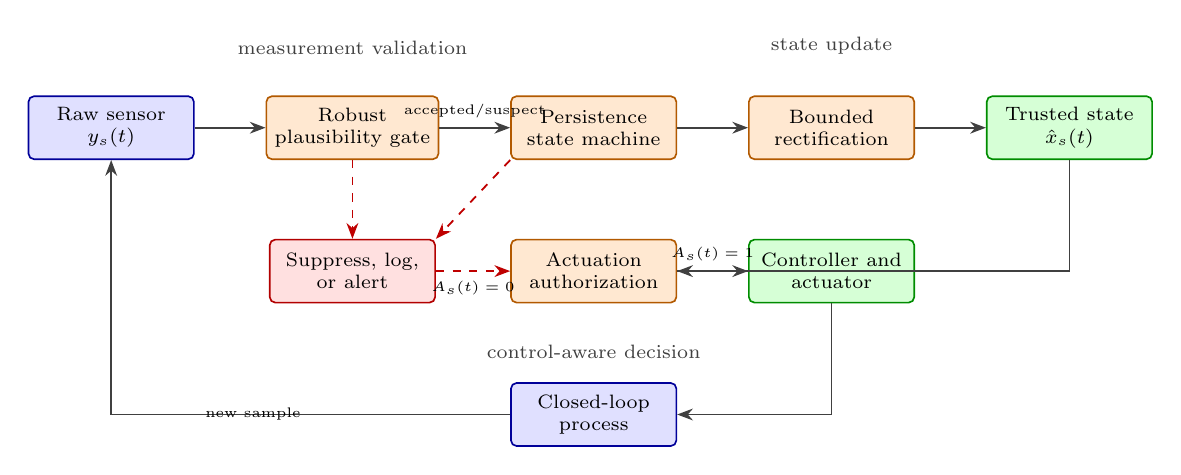
\begin{tikzpicture}[node distance=7mm and 9mm]
\tikzset{
  block/.style={rectangle, rounded corners=2pt, draw=black!70, line width=0.6pt,
    minimum width=21mm, minimum height=8mm, align=center, font=\scriptsize, inner sep=3pt},
  input/.style={block, fill=blue!12, draw=blue!60!black},
  module/.style={block, fill=orange!18, draw=orange!70!black},
  output/.style={block, fill=green!16, draw=green!55!black},
  danger/.style={block, fill=red!12, draw=red!70!black},
  flow/.style={-{Stealth[length=2mm,width=1.5mm]}, line width=0.65pt, draw=black!75},
  suppress/.style={-{Stealth[length=2mm,width=1.5mm]}, dashed, line width=0.65pt, draw=red!75!black},
  note/.style={font=\scriptsize, align=center, text=black!75}
}

\node[input] (raw) {Raw sensor\\$y_s(t)$};
\node[module, right=of raw] (gate) {Robust\\plausibility gate};
\node[module, right=of gate] (state) {Persistence\\state machine};
\node[module, right=of state] (rect) {Bounded\\rectification};
\node[output, right=of rect] (trusted) {Trusted state\\$\hat{x}_s(t)$};

\node[module, below=10mm of state] (auth) {Actuation\\authorization};
\node[output, right=of auth] (act) {Controller and\\actuator};
\node[input, below=10mm of auth] (process) {Closed-loop\\process};
\node[danger, below=10mm of gate] (fault) {Suppress, log,\\or alert};

\draw[flow] (raw) -- (gate);
\draw[flow] (gate) -- node[above, font=\tiny] {accepted/suspect} (state);
\draw[flow] (state) -- (rect);
\draw[flow] (rect) -- (trusted);
\draw[flow] (trusted.south) |- (auth.east);
\draw[flow] (auth) -- node[above, font=\tiny] {$A_s(t)=1$} (act);
\draw[flow] (act.south) |- (process.east);
\draw[flow] (process.west) -| node[pos=0.25, left, font=\tiny] {new sample} (raw.south);

\draw[suppress] (gate.south) -- (fault.north);
\draw[suppress] (state.south west) -- (fault.north east);
\draw[suppress] (fault.east) -- node[below, font=\tiny] {$A_s(t)=0$} (auth.west);

\node[note, above=4mm of gate] {measurement validation};
\node[note, above=4mm of rect] {state update};
\node[note, below=4mm of auth] {control-aware decision};
\end{tikzpicture}
}
\caption{Architecture of AASVR. Raw measurements first pass through robust plausibility gates that check physical range, local rate, trusted-state deviation, and uncommanded trends. Accepted or suspect readings then update a persistence state machine, which decides whether the trusted state should be updated, held, or rectified by a bounded prediction. Only trusted out-of-band states can authorize actuation. Rejected or fault-alert readings are logged and may trigger maintenance alerts, but they do not directly drive the actuator.}
\label{fig:architecture}
\end{figure*}

\subsection{Robust plausibility gate}
For each sensor, AASVR estimates a robust scale over adjacent changes,
\begin{equation}
\sigma_{\Delta,s}(t)=1.4826\,\mathrm{MAD}\left(\Delta y_s(t-w:t)\right).
\end{equation}
The accepted deviation tolerance is
\begin{equation}
\xi_s(t)=\max(\xi_{s,\min},c_s\sigma_{\Delta,s}(t),r_s\Delta t,u_s).
\end{equation}
A reading must satisfy broad physical range, maximum rate, and trusted-state deviation gates. A separate trend guard rejects slow monotonic movement when no relevant actuator activity explains the direction of change.

\subsection{State-machine persistence logic}
Figure~\ref{fig:state_machine} shows the five persistence states. A single failed gate moves a sensor into a suspect transient state. Repeated failures create a persistent-deviation state. Consistent evidence can be accepted as a new process regime, while missing, stuck, saturated, or contradictory readings escalate to fault alert.

\begin{figure}[t]
\centering
\resizebox{0.98\linewidth}{!}{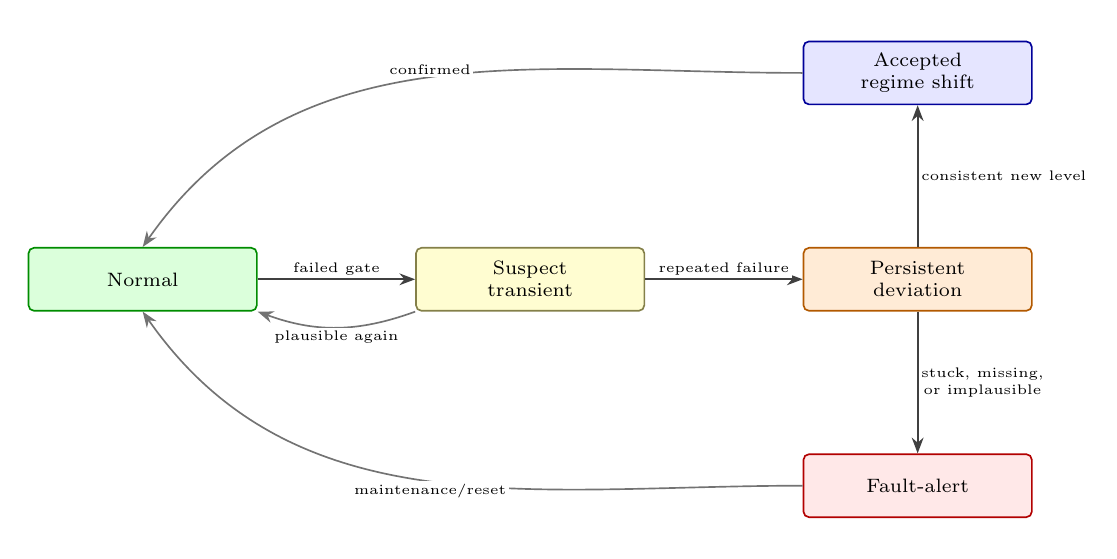
\begin{tikzpicture}[node distance=18mm and 20mm]
\tikzset{
  statebox/.style={rectangle, rounded corners=2pt, draw=black!70, line width=0.6pt,
    minimum width=29mm, minimum height=8mm, align=center, font=\scriptsize, inner sep=3pt},
  normal/.style={statebox, fill=green!14, draw=green!55!black},
  suspect/.style={statebox, fill=yellow!18, draw=yellow!45!black},
  persistent/.style={statebox, fill=orange!16, draw=orange!70!black},
  accepted/.style={statebox, fill=blue!10, draw=blue!60!black},
  fault/.style={statebox, fill=red!9, draw=red!70!black},
  flow/.style={-{Stealth[length=2mm,width=1.5mm]}, line width=0.65pt, draw=black!75},
  back/.style={-{Stealth[length=2mm,width=1.5mm]}, line width=0.6pt, draw=black!55},
  lab/.style={font=\tiny, align=center, fill=white, inner sep=1pt}
}

\node[normal] (normal) {Normal};
\node[suspect, right=of normal] (suspect) {Suspect\\transient};
\node[persistent, right=of suspect] (persistent) {Persistent\\deviation};
\node[accepted, above=of persistent] (accepted) {Accepted\\regime shift};
\node[fault, below=of persistent] (fault) {Fault-alert};

\draw[flow] (normal) -- node[lab, above] {failed gate} (suspect);
\draw[flow] (suspect) -- node[lab, above] {repeated failure} (persistent);
\draw[flow] (persistent) -- node[lab, right] {consistent new level} (accepted);
\draw[flow] (persistent) -- node[lab, right] {stuck, missing,\\or implausible} (fault);
\draw[back] (suspect.south west) to[out=-160,in=-20] node[lab, below] {plausible again} (normal.south east);
\draw[back] (accepted.west) to[out=180,in=55] node[lab, above] {confirmed} (normal.north);
\draw[back] (fault.west) to[out=180,in=-55] node[lab, below] {maintenance/reset} (normal.south);
\end{tikzpicture}
}
\caption{AASVR state machine. The state machine prevents one failed sample from immediately becoming a maintenance alert, but also prevents repeated failed samples from silently entering the controller. The accepted-regime-shift path allows real process changes to be incorporated after confirmation. The fault-alert path blocks single-sensor actuation authorization until maintenance, reset, or independent evidence restores trust.}
\label{fig:state_machine}
\end{figure}

\subsection{Rectification and actuation authorization}
When a reading is accepted, AASVR sets $\hat{x}_s(t)=y_s(t)$. When it is suspect, the method either holds $\hat{x}_s(t-1)$ or applies a bounded update limited by $r_s\Delta t$. Actuation is authorized only if the trusted value is outside the control band, the violation persists for the configured number of samples, the sensor state is normal or accepted-regime-shift, the trust score is sufficient, and the actuator is not in cooldown.

\begin{algorithm}[t]
\caption{Streaming AASVR update for one sensor}
\label{alg:aasvr}
\begin{algorithmic}[1]
\REQUIRE Raw value $y_s(t)$, previous trusted state $\hat{x}_s(t-1)$, recent history, limits, actuator state.
\STATE Estimate robust local scale $\sigma_{\Delta,s}(t)$ and tolerance $\xi_s(t)$.
\STATE Apply physical-range, rate, trusted-deviation, missingness, and trend gates.
\STATE Update the persistence state from the gate outcome.
\IF{the reading is accepted}
  \STATE Set $\hat{x}_s(t)\leftarrow y_s(t)$.
\ELSIF{the reading is transient suspect}
  \STATE Hold or bounded-predict $\hat{x}_s(t)$.
\ELSE
  \STATE Keep the last safe estimate and log a fault-alert decision.
\ENDIF
\STATE Authorize actuation only if trusted state, persistence, score, and cooldown rules are satisfied.
\RETURN Trusted value, sensor state, trust score, actuation flag, and log record.
\end{algorithmic}
\end{algorithm}

\section{Materials and Evaluation Protocol}
\subsection{Hydroponic deployment data}
The hydroponic data contain 121244 raw rows collected from 2024-02-27 to 2024-03-28 at a median cadence of approximately 16 seconds. The primary analysis uses electrical conductivity, pH, humidity, air temperature, water temperature, and carbon dioxide. Water level is excluded because the available raw values are not defensibly calibrated.

\subsection{External benchmarks}
HAI 21.03 and SKAB are used as public external stress tests. HAI labels are timestamp-level attack indicators over an industrial-control testbed. SKAB labels are timestamp-level anomaly indicators over process-loop experiments. For these datasets, a timestamp is predicted abnormal when at least 30\% of sensor streams reject or alert. We also report a threshold sensitivity sweep from 10\% to 90\%.

\subsection{Baselines and metrics}
The baselines are raw thresholding, the original manuscript method, moving average, moving median, Hampel, Kalman, EWMA, CUSUM, and PCA-style monitoring. The hydroponic synthetic-fault benchmark reports precision, recall, specificity, balanced accuracy, event recall, detection delay, false alarm events, and false actuation. Native-label external benchmarks report timestamp-level precision, recall, specificity, and balanced accuracy.

\section{Results}
\subsection{Hydroponic synthetic-fault benchmark}
Table~\ref{tab:hydro_synth} summarizes the primary target-domain result. AASVR achieved the highest balanced accuracy and the lowest mean false-actuation count among the compared methods. The absolute precision is low because the injected faults occupy a small fraction of all sensor-samples, so balanced accuracy, recall, specificity, and false actuation are more informative for the control-safety question.

\begin{table}[t]
\centering
\caption{Hydroponic synthetic-fault benchmark. The table reports the top methods by balanced accuracy on injected faults over the real hydroponic signal background. AASVR has the highest balanced accuracy and greatly fewer false actuations than the conventional filtering baselines.}
\label{tab:hydro_synth}
\begin{tabular}{lrrrrr}
\toprule
Method & Recall & Specificity & Bal. acc. & FPR & False act. \\
\midrule
AASVR & 0.839 & 0.880 & 0.859 & 0.120 & 0.145 \\
Kalman & 0.591 & 0.820 & 0.706 & 0.180 & 3.029 \\
PCA & 0.353 & 0.980 & 0.667 & 0.020 & 3.060 \\
Hampel & 0.353 & 0.980 & 0.667 & 0.020 & 3.038 \\
CUSUM & 0.344 & 0.987 & 0.666 & 0.013 & 3.060 \\
Original & 0.161 & 0.998 & 0.579 & 0.002 & 3.060 \\
\bottomrule
\end{tabular}
\end{table}

\begin{figure}[t]
\centering
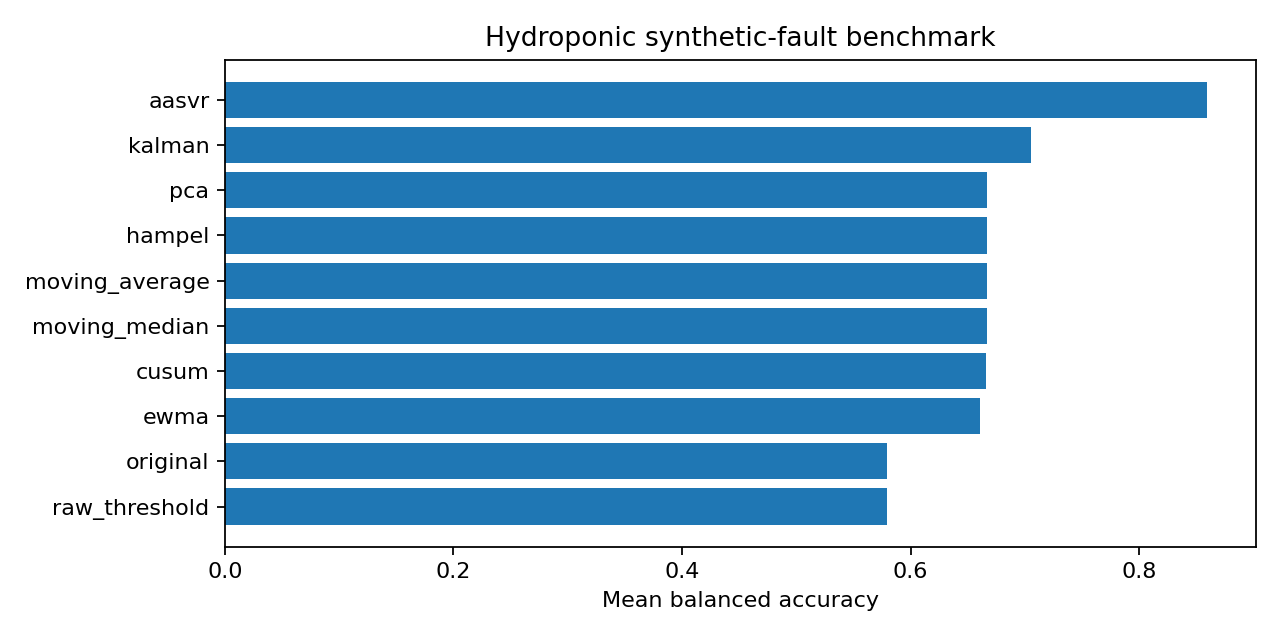
\includegraphics[width=0.82\linewidth]{figure/hydro_exp1_synthetic_balanced_accuracy.png}
\caption{Hydroponic synthetic-fault balanced accuracy across methods. The comparison is computed on repeated injected faults over windows sampled from the real hydroponic data. AASVR ranks first because it maintains high recall while preserving enough specificity to avoid passing many injected faults into the controller.}
\label{fig:hydro_bar}
\end{figure}

\begin{figure}[t]
\centering
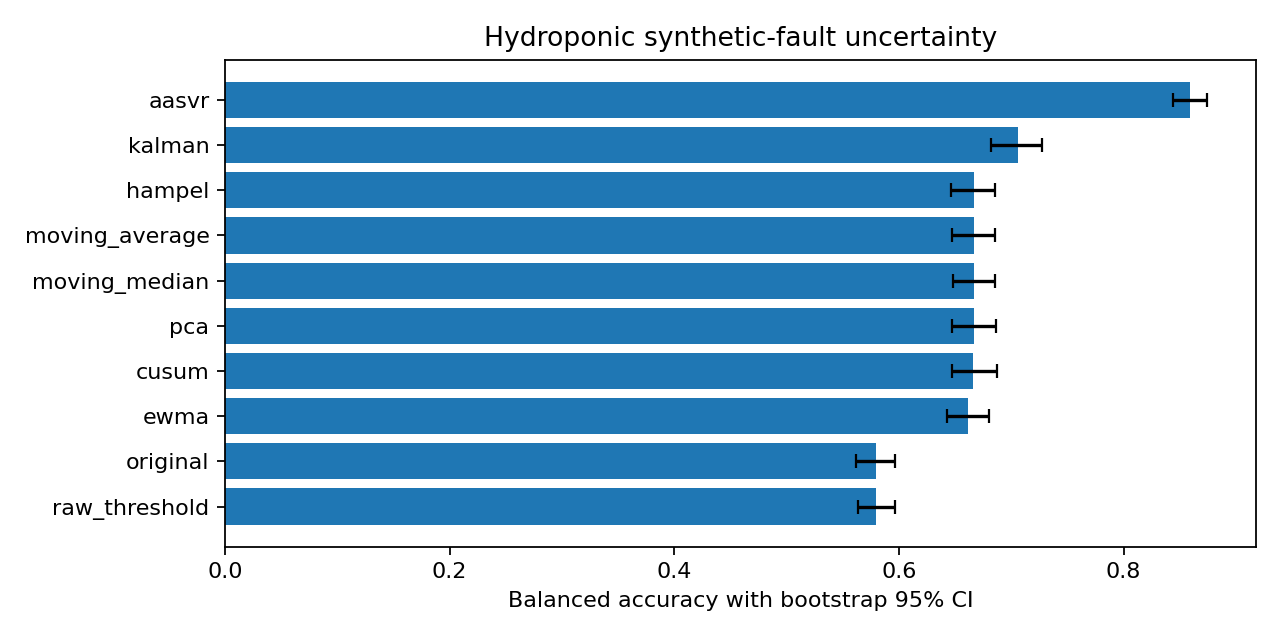
\includegraphics[width=0.82\linewidth]{figure/hydro_exp1_balanced_accuracy_ci.png}
\caption{Bootstrap uncertainty for hydroponic synthetic-fault balanced accuracy. AASVR reached a mean balanced accuracy of 0.859 with a 95\% bootstrap confidence interval of 0.844--0.874. The interval separates AASVR from the conventional baselines in the current benchmark, but the result remains tied to the injected fault model and available hydroponic trace.}
\label{fig:hydro_ci}
\end{figure}

\subsection{Ablation and control effect}
Table~\ref{tab:ablation} shows that several ablations preserve the same detection score but change control behavior. Removing actuation confirmation increases false actuation from 0.145 to 0.569 events per trial. This is the clearest evidence that AASVR is not only a detector: the actuation-aware layer changes downstream control outcomes.

\begin{table}[t]
\centering
\caption{AASVR ablation summary. Detection scores can remain similar while control-safety outcomes change. In particular, removing actuation confirmation leaves balanced accuracy unchanged but increases false actuation, which supports evaluating control-aware metrics rather than point-wise detection alone.}
\label{tab:ablation}
\begin{tabular}{lrrr}
\toprule
Variant & Bal. acc. & Recall & False act. \\
\midrule
Full AASVR & 0.859 & 0.839 & 0.145 \\
No actuation confirmation & 0.859 & 0.839 & 0.569 \\
No cooldown & 0.859 & 0.839 & 0.269 \\
No robust MAD scale & 0.854 & 0.864 & 0.133 \\
No trend guard & 0.843 & 0.801 & 0.260 \\
Bounded prediction mode & 0.810 & 0.734 & 0.476 \\
\bottomrule
\end{tabular}
\end{table}

\subsection{External benchmark performance}
Table~\ref{tab:external} reports the fixed 30\% native-label protocol for HAI and SKAB. AASVR ranks first on both datasets under this fixed rule, but the nature of the result differs. HAI has high specificity and modest recall, while SKAB has high recall and low specificity.

\begin{table}[t]
\centering
\caption{External native-label results under the fixed 30\% timestamp aggregation rule. The values should be read as cross-domain stress-test evidence rather than direct hydroponic fault evidence. HAI contains cyber-physical attack labels, while SKAB contains process-loop anomaly labels.}
\label{tab:external}
\begin{tabular}{llrrrr}
\toprule
Dataset & Method & Precision & Recall & Specificity & Bal. acc. \\
\midrule
HAI & AASVR & 0.078 & 0.404 & 0.929 & 0.667 \\
HAI & Kalman & 0.136 & 0.312 & 0.971 & 0.641 \\
SKAB & AASVR & 0.379 & 0.975 & 0.358 & 0.666 \\
SKAB & Kalman & 0.376 & 0.975 & 0.349 & 0.662 \\
\bottomrule
\end{tabular}
\end{table}

\begin{figure}[t]
\centering
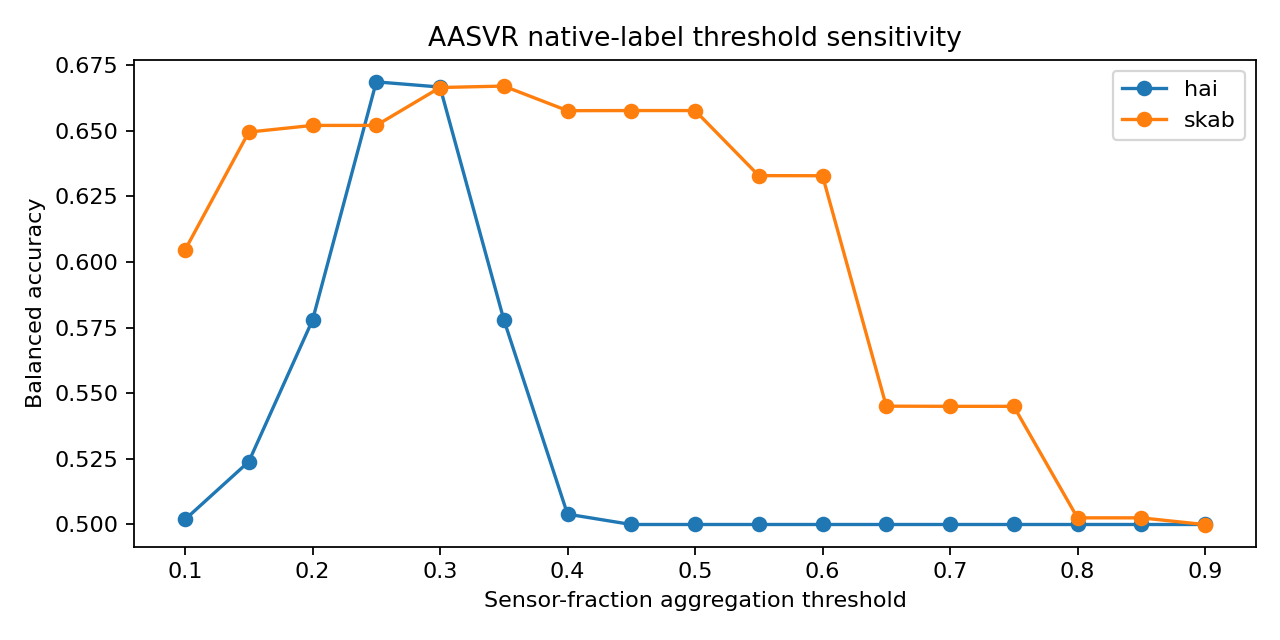
\includegraphics[width=0.84\linewidth]{figure/external_aasvr_threshold_sensitivity.png}
\caption{Threshold sensitivity for timestamp-level external labels. The fixed 30\% aggregation rule is the headline protocol, but this plot shows how AASVR changes when the required fraction of rejecting streams is varied. SKAB is stable around the headline setting, while HAI reveals a tradeoff between recall and specificity.}
\label{fig:threshold}
\end{figure}

\begin{figure}[t]
\centering
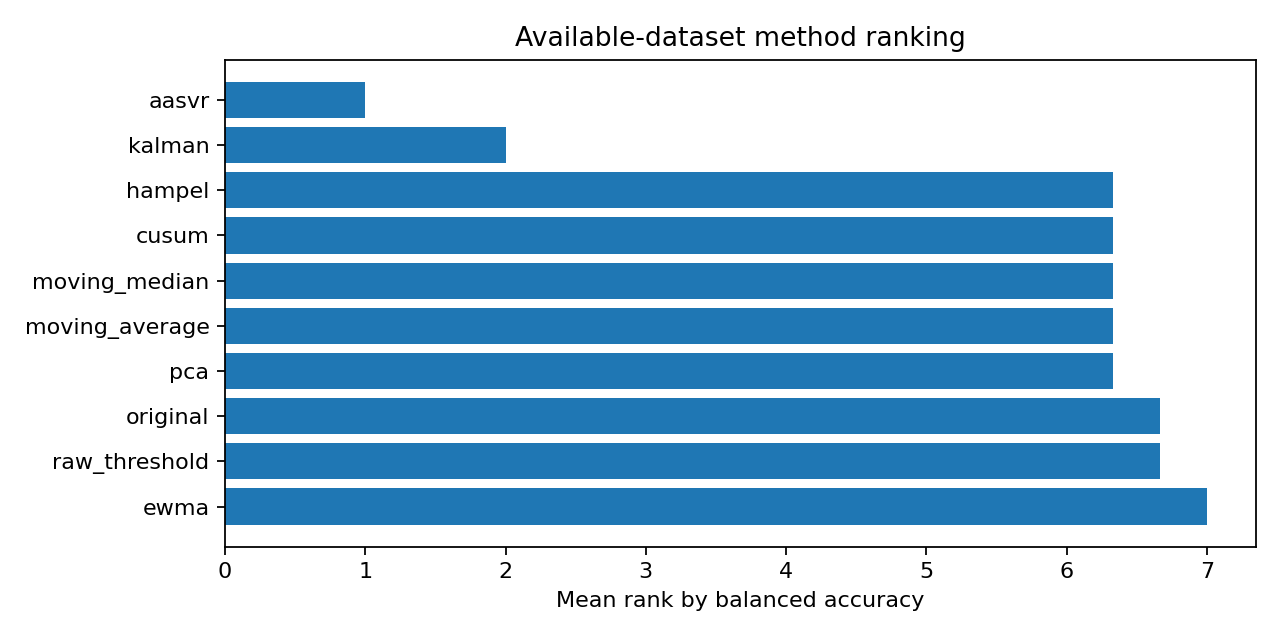
\includegraphics[width=0.82\linewidth]{figure/cross_dataset_rank_plot.png}
\caption{Mean rank by balanced accuracy across available benchmark tables. The ranking combines hydroponic synthetic faults with native-label external benchmark summaries. It is useful for orientation, but it should not be interpreted as a leaderboard because the datasets use different label semantics and evaluation units.}
\label{fig:rank}
\end{figure}

\subsection{Representative hydroponic trace}
Figure~\ref{fig:ph_trace} shows a pH replay segment. The trace is included to connect the aggregate benchmark to the actual deployment setting. It illustrates the measurement-to-state transformation that precedes any actuation decision.

\begin{figure}[t]
\centering
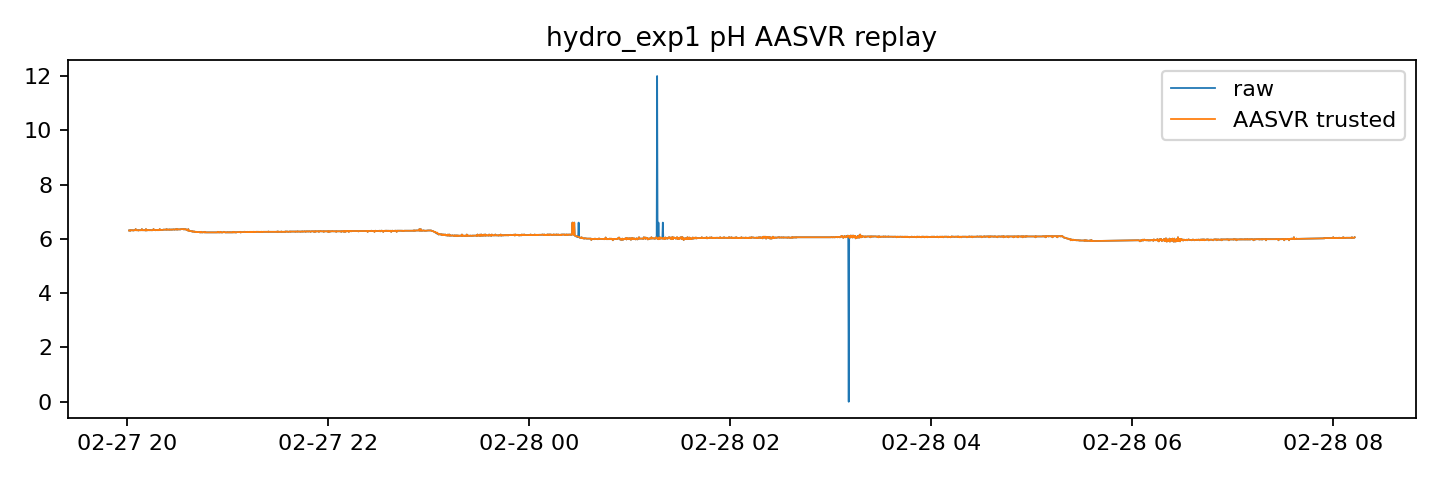
\includegraphics[width=0.9\linewidth]{figure/hydro_exp1_ph_trace.png}
\caption{Representative pH replay from the hydroponic deployment data. The raw stream and AASVR trusted estimate are plotted over an early segment of the experiment. The figure is not used as a ground-truth fault label; it is included to show how the method exposes a trusted state rather than passing every raw measurement directly to the controller.}
\label{fig:ph_trace}
\end{figure}

\section{Discussion}
\subsection{Why actuation awareness matters}
The ablation results show why actuation-aware validation should be evaluated with control metrics. A detector can produce the same point-wise score while changing the number of authorized actuator events. For hydroponic systems, this distinction is practical because unnecessary dosing or cooling can disturb the process even if the signal-level anomaly score appears acceptable.

\subsection{Cross-domain generalization}
The external benchmark results support a cautious generalization claim. AASVR can run on independent industrial-control and process-loop datasets with the same streaming interface. However, HAI attacks and SKAB process anomalies are not identical to low-cost hydroponic sensor faults. The external results therefore test robustness of the validation principle, not agronomic performance.

\subsection{Limitations}
The hydroponic experiment does not provide independent reference instruments for every sensor at every time point. Synthetic fault injection is therefore necessary for controlled scoring, but injected faults cannot cover every real failure mode. The external datasets use timestamp-level labels, so the multivariate aggregation threshold affects the result. Crop outcomes are treated only as deployment context because enclosure, lighting, cooling, nutrient delivery, carbon dioxide regulation, and automation are confounded.

\section{Conclusion}
We proposed AASVR, an actuation-aware sensor validation and rectification method for closed-loop measurement and control systems. The method separates validation, state update, rectification, and actuation authorization so that untrusted measurements can be logged without directly driving the controller. On hydroponic synthetic faults, AASVR improved balanced accuracy and reduced false actuation compared with conventional baselines. Public SKAB and HAI benchmarks show that the same interface transfers to external process data, while also exposing threshold-dependent tradeoffs that should be reported rather than hidden.

\section*{Data Availability}
The repository contains code, configuration files, processed-data descriptors, Docker workflow files, and paper-generation assets. Raw hydroponic and external benchmark files are not committed to the repository. Public datasets can be obtained from their original providers, and request-access datasets should be obtained under the providers' terms.

\section*{Declaration of Competing Interest}
The authors declare no competing interests for the current manuscript draft.

\section*{Declaration of Generative AI and AI-Assisted Technologies}
AI-assisted tools were used to help organize code, draft text, and check consistency. The authors remain responsible for the scientific content, claims, results, and final manuscript.

\bibliographystyle{elsarticle-num}
\bibliography{aasvr_references}

\end{document}
